% Set a sane document class, 12pt font, and a report template
\documentclass[a4paper, twoside, openright, 12pt]{report}

% Import used packages
\usepackage{graphicx}
\usepackage{hyperref}
\usepackage{listings}
\usepackage{longtable}
\usepackage{lscape}
\usepackage{parskip}
\usepackage{color}
\usepackage{multirow}
%\usepackage[lmargin=25mm,rmargin=25mm,tmargin=40mm,bmargin=30mm]{geometry}
\usepackage{setspace}
\usepackage{fancyhdr}
\usepackage{multicol}
\usepackage[x11names, rgb]{xcolor}
\usepackage[utf8]{inputenc}
\usepackage{tikz}
\usetikzlibrary{decorations,arrows,shapes}
\usepackage{amsmath}



% Bibliographies
\usepackage[defernumbers=true]{biblatex}
\bibliography{bibliography}

% Use UTF-8
%\usepackage[utf8x]{inputenc}
\def \authors {Ken B\o{}rge Melhus Viktil \& Martin Tobias Holmedahl Sandsmark}
\def \papertitle {Jantu - A Cognitive Agent Playing StarCraft: Brood War}

% Meta-information for the PDF
\hypersetup{
pdfauthor = \authors,
pdftitle = \papertitle,
pdfsubject = {Master project for IDI},
pdfkeywords = {project, cognitive, architecture, starcraft, artificial
    intelligence},
pdfcreator = {LaTeX with hyperref package lol},
pdfproducer = {pdflatex}}

%opening
\title{\papertitle}
\author{\authors}

\begin{document}

% Abstract in english
\begin{abstract}
It has been shown that most players enjoys playing video games against other human players instead of computer controlled opponents. But most research on artificial intelligence in gaming today focus on just winning in the most effective way possible, instead of making the agents more human-like.

Cognitive architectures are designed to emulate how the human brain operates when performing tasks. Very little research has been done on applying cognitive methods to the field of real-time strategy games.

In this paper we aim to research the use of a cognitive model that is capable of playing StarCraft: Brood War with decent results. The result is an AI agent implemented with a cognitive framework called LIDA. The resulting agent is only a proof of concept implementation, but we provide suggestions for how it can be improved in the future, and where the problems and limitations of our approach lies.
\end{abstract}
\thispagestyle{empty}
\cleardoublepage

% Abstract in norwegian
\renewcommand{\abstractname}{Sammendrag}
\begin{abstract}
Det har vist seg at folk som spiller spill foretrekker å spille mot andre mennesker, i motsetning til å spille mot kunstige spillere, men størstedelen av forskningen på kunstig intelligens i spill i dag fokuserer mer på å vinne mest mulig effektivt, istedenfor å se på hvordan man kan få de til å spille mer menneskelig.

Kognitive arkitekturer er laget for å emulere hvordan den menneskelige hjernen utfører oppgaver. Det er per dags dato nesten ikke noe forskning på bruk av kognitive arkitekturer innen sanntidsstrategispill.

I denne teksten vil vi undersøke bruken av en kognitiv modell for å spille StarCraft: Brood War. Resultatet er en agent implementert med programvarerammeverket LIDA. Agenten er en prototypeimplementasjon, men vi kommer også med forslag til hvordan den kan forbedres i fremtiden, og hvilke problemer og begrensninger tilnærmingen vår har.
\end{abstract}
\thispagestyle{empty}
\cleardoublepage

% Acknowledgements
\renewcommand{\abstractname}{Acknowledgements}
\begin{abstract}
Firstly we would like to thank our supervisors; Helge Langseth and Anders Kofod-Petersen. We would also like to thank the Cognitive Computing Research Group at the University of Memphis, for their LIDA framework which is the basis of our project. Finally we would like to thank the developers of the BWAPI project, and in particular Adam Heinermann, as well as the rest of the members in the \#BWAPI IRC channel on Freenode.
\end{abstract}
\thispagestyle{empty}
\cleardoublepage

\pagenumbering{roman}

% TOC
\tableofcontents
\cleardoublepage

% Figures
\listoffigures
\cleardoublepage

% Tables
\listoftables
\cleardoublepage


% Content
\pagestyle{fancy}
\pagenumbering{arabic}

%!TEX root = main.tex

\chapter{Introduction}
In this chapter we introduce our project, as well as the background and
motivation for doing this. Section \ref{sec:background} presents the background
and our motivation for the project, a short introduction to Starcraft and the
API we will use and describes what we will do in this project and our main
goals. Section \ref{sec:contributions} contains the main contributors to the
project as well as our supervisors. Section \ref{sec:goals} explains the goals we hope to accomplish during the project. 
Section \ref{sec:structure} introduces the
structure of this report.

\section{Background and Motivation}
\label{sec:background}
It is our opinion that the study of cognitive architectures are woefully underrepresented in the field of artificial intelligence, and also in the domain of computer games. We believe that the use of cognitive architectures should be further explored to attain a better understanding of the gains from using a cognitive architecture.

\section{Name}
\label{sec:name}
The name {\em Jantu} is hindi, and is translated as ``Pertaining to the merely sentient part of a creature, as distinguished from the intellectual, rational, or spiritual part; as, the animal passions or appetites.'', which reflects what we are trying to achieve with our work in this project.\cite{hindijantu}

\section{Contributions}
\label{sec:contributions}
Firstly we would also like to thank our supervisors; Helge Langseth and Anders Kofod-Petersen. We would also like to thank the Cognitive Computing Research Group at the University of Memphis, for their LIDA framework which is the basis of our project.

\section{Project goals}
\label{sec:goals}
First and foremost we set out to create a proof of concept agent that could play the game StarCraft: Brood War, built using a cognitive architecture.

Secondly we want to explore what problems one faces when using a cognitive architecture in this domain, but also what works well.

\section{Report Structure}
\label{sec:structure}
This report is structured into four chapters:
\begin{itemize}
\item Chapter 1: \textbf{Introduction} \\
This chapter describes the motivation and goal of the project as well as who
contributed and the general structure of the report.
\item Chapter 2: \textbf{Theory} \\
In this chapter we present the domain we're working in; the real-time computer strategy game StarCraft: Brood War. We also present the cognitive architecture we're using.
\item Chapter 3: \textbf{Implementation} \\
This chapter presents our implementation.
\item Chapter 4: \textbf{Results} \\
This chapter presents how our implementation performed.
\item Chapter 5: \textbf{Evaluation} \\
Here we summarize and evaluate the work presented in this report.
\item Chapter 6: \textbf{Future Work} \\
Here we give some ideas of what work is left, and where others can build on our project to make it better.

\end{itemize}
%!TEX root = main.tex

\chapter{Theory}
In this chapter we will the present theory that is important for our project. In addition to a general eplaination of the game, we also explain the BWAPI architecture, and how it utilizes shared memory and JNI to allow bots written in Java. Section \ref{sec:cogarch} describes the models of cognition and the theory behind them and a description it is. Section \ref{sec:lida} describes the LIDA model of cognition.
%!TEX root = main.tex

\section{StarCraft}
\label{sec:starcrafttheory}


\begin{figure}[h!tb]
\centering
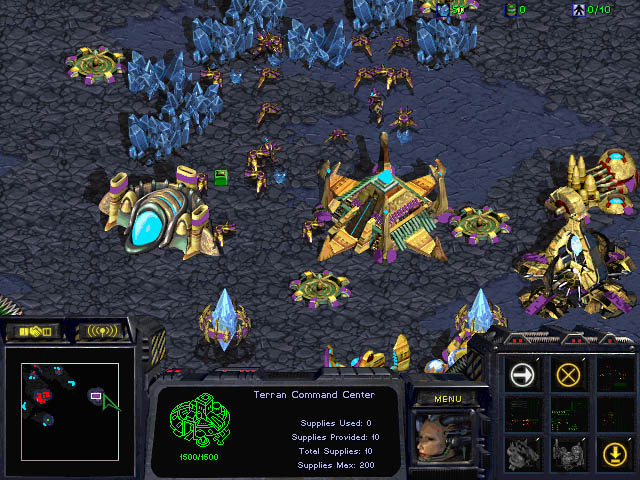
\includegraphics[scale=0.5]{graphics/scbw.jpg}
\caption{StarCraft: Brood War}
\label{fig:scbwIntro}
\end{figure}
%General introduction to the game, with emphasis on the parts that we utilize most in our project

StarCraft is a multi-player, real-time strategy (henceforth referred to as RTS) game, with a heavy focus on both economic strategies, as well as effective management of individual in-game units. Brood War is the expansion pack for the original StarCraft game that introduced new units, maps and upgrades. The game has been praised for its emergent complexity even though the mechanics are simple to understand. Brood Wars has been played on a high competetive level for over 10 years, and it has been evolving all that time with new strategies and tactics.

\subsection{Races}
The game has three races that a player selects between. The insect race Zerg, the advanced alien race Protoss and the humans Terran. Each race has it's own units and buildings as well as different game mechanics. 

\subsubsection{Terran}
\begin{figure}[h!tb]
\centering

\includegraphics[scale=0.7]{graphics/terranicon.png}
\caption{The in-game logo of the Terran race.\cite{terranlogo}}
\end{figure}

The terran are human colonists originally from earth. This is the most balanced race, which relies on a mixture of large numbers and powerful units. They have great mobility in their biological armies, and  great defense and slow turtling in their mechanical units like tanks. 

The Terran worker is a Space Construction Vehicle (SCV), and unique for Terran is that is can repair any mechanical unit or buildings if they get damaged.

Another unique mechanic with Terran is that their buildings can lift of and fly around to reposition themselves.

Several of the buildings can also be upgraded with addons that are smaller buildings that are constructed and connected to the main building. Addons unlock new upgrades and units to be constructed from the building it is connected to. Using lift off buildings can swap addons after they are constructed, so that opens up more possible build order diversity.

Every Terran unit can be healed after they take damage, the mechanical units and buildings can be repaired using an SCV, but doing so means that the worker will not be gathering resources for that time. To heal damaged biological units you have to train special units called Medics. 

\subsubsection{Zerg}
\begin{figure}[h!tb]
\centering

\includegraphics[scale=0.3]{graphics/zergicon.png}
\caption{The in-game logo of the Zerg race.\cite{zerglogo}}
\end{figure}

The zerg is an insect-like collection of different biological races assimilated under a central intelligence.

They rely on biological abilities that are selectively evolved as appose to using technology like the other two races.

The individual units in the Zerg army is not very powerful, but their strength lies in superior numbers of units as well as the ability to quickly reinforce the army with new units when some dies off.

The Zerg worker unit is called a drone, and what separates this worker from the other races is that in order to create a new building the worker has to sacrifice it self to morph into the new building.

Zerg has a unique game mechanic for creating new units. The main building, called the hatchery, creates larva on regular intervals, up to a maximum of three, that can be morphed into new units. Both workers and army units are created from the larva, and because of the limited availability on these a player has to prioritize at all time if he wants to create workers or army units.

To increase the production capacity they have to either expand to a new base, or create several hatcheries in their current bases to gain access to more larva.

Zerg can only build new buildings on creep, something that spreads from existing buildings as well as Creep Colonies, a special building that is used only for extending creep coverage on the map.

Zerg units have a unique ability to regenerate health after they are damaged if they get left alone out of combat. This makes retreating and regrouping a good tactic for zerg players as their army will have time to regenerate back to full health after a defeat on the battleground. Together with another unique ability some of the Zerg units have that is called burrow, that allows the to burrow under ground and hide or run away, it can be really hard to kill some units since they can escape and regenerate the lost health. 

\subsubsection{Protoss}
\begin{figure}[h!tb]
\centering

\includegraphics[scale=0.3]{graphics/protossicon.png}
\caption{The in-game logo of the Protoss race.\cite{protosslogo}}
\end{figure}

The protoss is a highly advanced race with powerful mental abilities.

They are both technologically and military advanced, and usually rely on few, but very powerful single units. They have very expensive units that can crush a much bigger army by themselves.

The protoss worker is called a probe, probes doesn't need to construct the buildings, they only tag an area and then the building gets warped in from the protoss home world. This means a single probe can start the construction of several buildings at the same time and then return to gathering resources.

Similar to Zerg, Protoss can't simply construct buildings anywhere, they have to be constructed on a power grid that is generated by pylons, the Protoss supply building.

A unique Protoss feature is that all the units and buildings have shields that protect them from damage and regenerates over time. For an enemy to damage the unit it first has to deplete the shield, then it can do damage to the health of the unit. But damage taken after the shield is down cannot be healed or repaired.

\subsection{Gameplay}
\subsubsection{Micro vs. macro}
Two well-known concepts in the RTS communities, and the StarCraft community in particular, are micro management and macro management. Macro management refers to large-scale economic and strategic decisions, while micro management refers to smaller-scale control of individual units, or groups of units.

A good control of both concepts is needed for a successful agent.

\subsubsection{Supply}
Supply is a term for an artificial limit imposed by the game on how many units a player is allowed to make at any time. To increase the supply, a player can build a special kind of units; for the Protoss race this is {\em pylons}, for Zerg it is {\em overlords} and for Terran it is {\em supply depots}. The name stems from the terran unit needed, supply depots.

\subsubsection{Fog of war and scouting}
Fog of war is a well-known term from RTS games, which denotes un-observed parts of the environment or map. In StarCraft this is shown as shaded on screen. This leads to partial observability, and gives rise to uncertainty about the rest of the map, about what the other player is doing and what resources he has exhausted. To counteract this, it is common to {\em scout}, that is, to send out units to simply observe the other player.

\subsection{BWAPI}
To ease the development of third-party agents that play the game, an application programming interface (API) has been developed for StarCraft: Brood War, by third-party developers. They have relied on reverse engineering of the original game for developing it. It works by injecting itself into the process of the game, and hooking into various functions used in the game, as well as reading various memory areas directly.\cite{bwapi}

There has sprung up a sizable community around this effort, and there are several tournaments where programmers can participate with their own agents.\cite{bwapi}\cite{sscait}

There are also several third-party addons and extra libraries for easing the development of agents, such as the Brood War Terrain Analyzer (BWTA), which provides easy-to-use functions for analyzing the maps for finding choke-points and suitable locations for various buildings,\cite{bwta} and the Brood War Standard Addon Library (BWSAL) which is both a generic, modular framework for BWAPI agents as well as default implementations for a large part of the modules needed for implementing such an agent.\cite{bwsal}

BWAPI only provides a C++ API, so for using it from other languages various types of bindings are needed.

There are two modes for loading agents using BWAPI; loading it directly into the StarCraft process, or using a shared-memory area to communicate state between the agent process and the StarCraft process in which the BWAPI code is running.\cite{bwapi}

\subsubsection{JNIBWAPI}
For using Java for developing an agent the most well-supported is using the JNIBWAPI project, which uses JNI to provide Java-bindings for BWAPI. It utilizes the shared-memory approach of BWAPI to avoid having to load the Java virtual machine into the StarCraft memory.

\section{Cognitive Architectures}
\label{sec:cogarch}
Cognitive architectures are architectures that base themselves on some model of human cognition. There are several competing theories about how cognition works, and one of the most recent and well-supported is the Global Workspace Theory.

One area that haven't been as well explored in relation to RTSes in general and StarCraft in particular, is cognitive architectures. Arrabales et al put forth that this is perhaps because of poor understanding within the field of classical AI of research into cognition\cite{arrabales2009gamechars}.

\subsection{Global Workspace Theory}

\begin{figure}[h!tb]
\centering
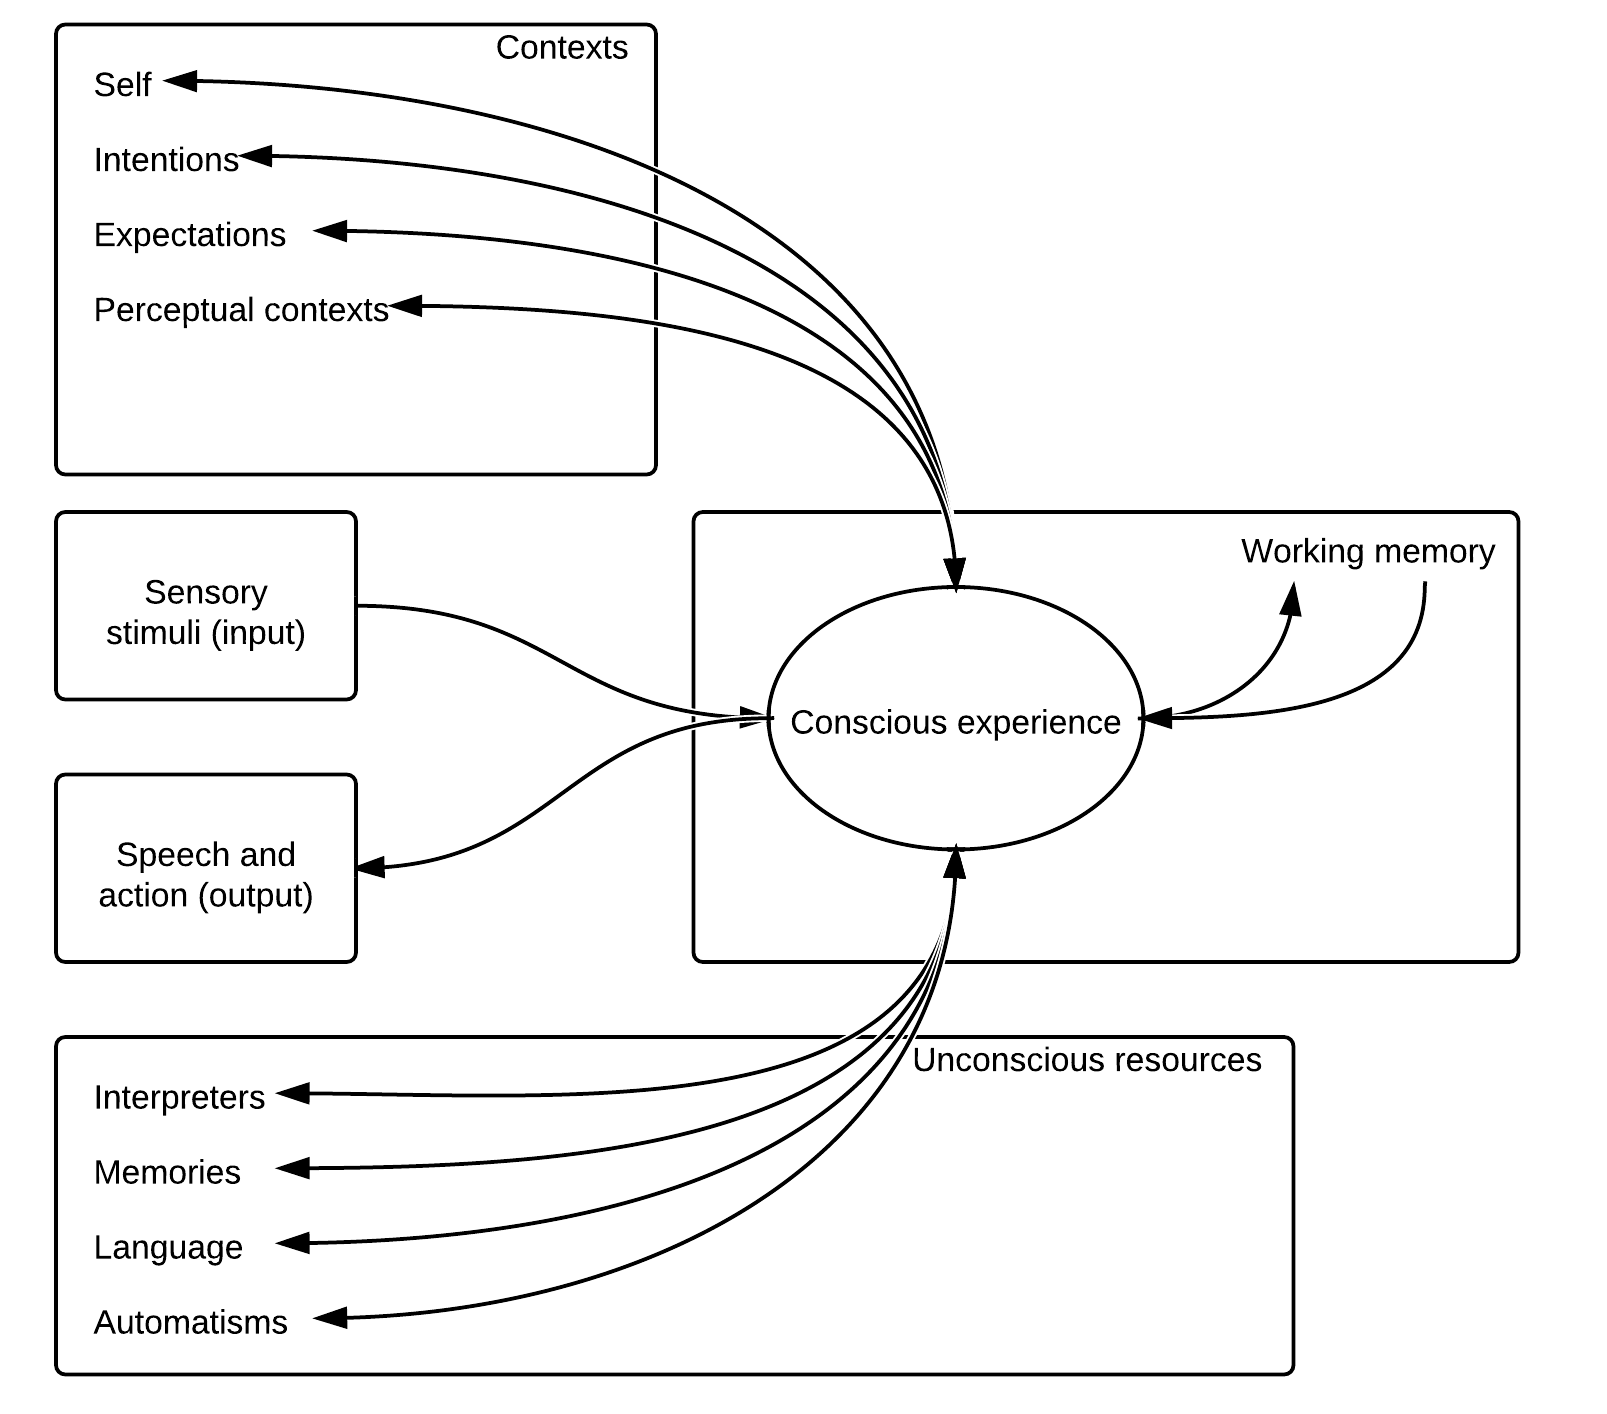
\includegraphics[scale=1.0]{graphics/globalworkspace.png}
\caption{A schematic of the Global Workspace theory\cite{baars2005gwt}}
\label{fig:gwt}
\end{figure}

Global Workspace Theory is a model of cognition that is very well supported by experimental data, and is one of the most widely accepted models. \cite{dehaene2001towards} It has been used to implement processes that imitate human decision making (for example for solving the problem of assigning people to jobs in the US Navy).\cite{baars2005gwt}\cite{franklin2003interacting}

It is based around an understanding of the brain as a set of many independently processing modules, working together by utilizing a shared workspace (hence the ``global workspace''). Every ``cognitive cycle'' all the processes compete for attention, and a single one gets the proverbial spotlight shone upon it.\cite{baars2005gwt}

There have been several implementations of GWT for different domains and approaches, for example the LIDA (``Learning IDA'') model\cite{franklin2007lida}, or the CERA-CRANIUM architecture\cite{arrabales2009ceracranium}.

See figure \ref{fig:gwt} for an overview of the theory.

\subsubsection{Neurological basis for the Global Workspace Theory}
According to \cite{llinas1998neuronal}, the looped neural pathways between the thalamus and the cortex might be what is responsible for the conscious collaboration between various parts of the brain. The thalamus is responsible for letting various parts of the cortex broadcast and influence the rest of the cortex. This meshes well with the global workspace theory, and the idea of a single subsystem broadcasting its contents to the rest of the whole.

There has also been discovered a link between the switching between coherent and decohoerent EEG-activity that seems to indicate a switching between states of competition for access to the global workspace. Decoherent electric activity seems to indicate a competitive process, while coherent activity indicates a passive ``listening''.\cite{freeman2003neurobiological}

The periods between these states is compatible with the widely accepted figures for the time it takes for stimulus to become conscious.\cite{shanahan2005applying}

Several studies have support the theory that consciousness is what enables global activation. They usually compare conscious and unconscious conditions in conscious subjects. Either by sensory stimulation or {\em overpractice of automatic habits}, that is; consciously doing tasks that usually are done unconsciously. All results show that conscious processes lead to widespread cortical activation, while unconscious ones usually only activates local regions.\cite{baars2003brain}

There has also been experiments done where subjects have been in various states of unconsciousness (sleep, general anasthesia, epileptic loss of consciousness and vegetative states), and it has been found that sensory stimulation in all states only lead to local activation in the cortex.\cite{shanahan2005applying}

\subsubsection{Implementations}
There has been implementations of several architectures incorporating the global workspace theory, and several other psychological theories.

\paragraph{IDA}
In the mid-nineties an artificial agent was designed for the U. S. Navy that would replace so-called ``detailers'', which are specialists that allocate personell. They take into account personal preferences, moving costs, requirements from the Navy (number of personell on each boat etc.) and various regulations from the Navy. Preferences from sailors are taken in from natural language e-mails, and these are processed using a slipnet that processes the natural language into something that has usable semantic meaning for the system. The other inputs (regulations and requirements from the Navy, e. g.) are stored in databases, and are pre-processed by similar slipnets before being pushed into the system. This system is able to replace the 300 or so detailers that the Navy employs. The system is up and running, and is matching the performance of the human detailers. \cite{baars2007architectural}\cite{franklin1998ida}

\paragraph{LIDA}
One problem with IDA was that learning wasn't really implemented at all, and therefore they started re-implementing from scratch, in a project called LIDA, for the Learning IDA system. The idea was to add learning from experience; learning newly perceived objects and their relationships to already known objects, relationships between objects, categories, relationships between objects and actions, effects of actions, and improved perception/tagging of sensory data with learned memories.\cite{franklin2006lida} Over time, however, LIDA evolved to become a more generic Java-framework for cognitive architectures.\cite{snaider2011lida}

\paragraph{CERA-CRANIUM}
This is a two-fold architecture, as reflected in the name. {\em CRANIUM} is a more generic tool for creation of a high amount of parallel processes operating with shared workspaces. {\em CERA} uses these services for creating a dynamic and adaptable system which operates on perceptions and generates actions, based on a cognitive model.\cite{arrabales2009gamechars} It has been used for making agents that act in several different environments, both virtual environments like the computer game Unreal Tournament, as well as real environments, where it has been embodied in small robots that map out unknown environments. \cite{arrabales2009ceracranium}

\subsection{Cognitive Models in Game AIs}
There have been several more or less successful attempts at implementing models of cognition into game-playing agents. Examples of this is CERA-CRANIUM, which was used to implement an agent playing Unreal Tournament \cite{arrabales2009ceracranium}, and SORTS which implemented an agent for the real-time strategy game ORTS using the symbolic, cognitive architecture Soar.\cite{wintermute2007sorts} One of the reasons for using computer games for experiments with regards to high-level artificial intelligence is that the characteristics of computer games lend themselves to this, by eliminating noise and uncertainty, and providing a more or less realistic simulated environment.

\subsubsection{SORTS}
%!TEX root = main.tex

\section{LIDA}
\label{sec:lida}
LIDA is both the name of a cognitive model and a software framework based on the cognitive model. Both are developed at the Cognitive Computing Research Group\footnote{\href{http://ccrg.cs.memphis.edu/}{\tt http://ccrg.cs.memphis.edu/}} at the University of Memphis. The LIDA framework is currently in beta, but it is based on the well-tested IDA project.

\subsection{The LIDA model}
\begin{figure}[h!tb]
\centering
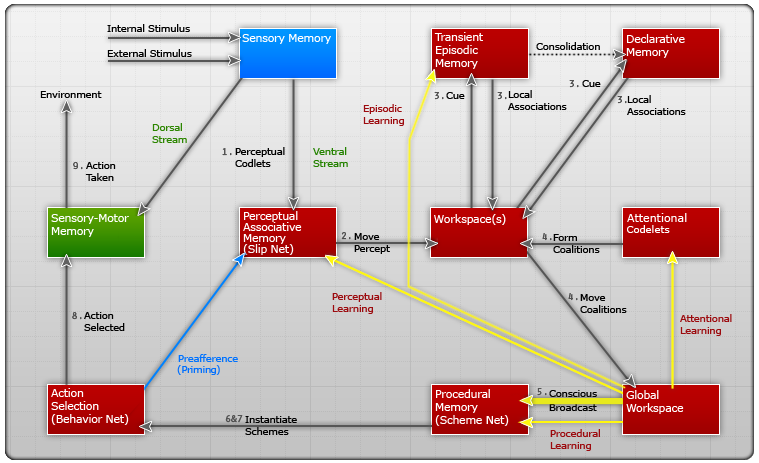
\includegraphics[width=\textwidth]{graphics/lida-model.png}
\caption{Overview of the LIDA cycle.\cite{franklin2007lida}}
\label{fig:lida-cycle}
\end{figure}

The LIDA model is a conceptual and computational model that describes cognition. It is based on the General Workspace Theory, which is a theory to describe functional consciousness. It incorporates and accounts for a large number of psychological and neuropsychological theories.\cite{Franklin2012}

\subsubsection{The LIDA cognitive cycle}
The computational model of LIDA views the artificial agent's ``life'' as a series of cognitive cycles. A high-level, simplified view of how this cognitive cycle is modeled in LIDA can be seen in figure \ref{fig:lida-cycle}. The cognitive cycle itself is subdivided into three separate phases; the understanding phase, the consciousness phase and the action selection phase.

\paragraph{Understanding phase}
In the understanding phase sensory input is tagged with semantic meaning. First low-level feature detectors in the Sensory Memory are run on the incoming stimuli. The output from these is passed onto the Perceptual Associative Memory. There higher-level feature detectors are run, which recognise abstracted entities like objects, events, actions, etc. The output of these is sent to the Workspace, from where it is pushed to both the Transient Episodic Memory and the Declarative Memory. Local associations generated from these memory modules are combined with the percept to generate a Current Situational Model, which is the agent's ``inner map'' of how the world looks.
\paragraph{Attention phase} Parts of the Current Situational Model is composited together to coalitions by Attention Codelets. These coalitions are put into the Global Workspace. From the Global Workspace a codelet selects the coalition in most need of conscious attention and broadcasts this.
\paragraph{Action selection phase} The Action Selection module takes in possible action schemes (behaviours) from the Procedural Memory, and selects one of these according to a competetive process. The selected action scheme is sent to the Sensory-Motor Memory, where it is executed. This method of action selection is based on Maes' behaviour net.\cite{maes1989right} Learning is also done in the action selection phase. In the Perceptual Associative Memory new entities and associations are created and old ones are reinforced during this phase. In the Transient Episodic Memory events from the broadcast from the Global Workspace are stored. The Procedural Memory stores new possible action schemes from the broadcast, and reinforces old ones.


\subsubsection{The workspace}
The workspace is composed of three main modules; the Current Situational Model, Scratchpad and the Conscious Contents Queue.

\paragraph{Current Situational Model} This is where the internal ``map'' of the agent is represented. This contains current events that are linked to associations. Various structure-building codelets running in the Workspace are responsible for building these.
\paragraph{Scratchpad} The Scratchpad is used for temporary storage for the codelets while they build up structures before moving into Current Situational Model.
\paragraph{Conscious Contents Queue} This contains a list of previous broadcasts, which allows LIDA to take time into account, and reason on, things that happens over time.

\subsection{LIDA framework}
\subsubsection{Background}
The LIDA framework implements a growing subset of the full computational LIDA model in a re-usable Java-based software framework.

While LIDA seems to have started simply as an extension for the IDA agent with added learning modes\cite{franklin2007lida}, it has evolved into a generic AGI framework, which can be used for other models than LIDA, because of the modular nature of the framework.\cite{snaider2011lida}

The reason for using a framework is that software projects implementing cognitive models tend to grow fairly large and complex therefore difficult to both implement in the first place and maintain over time.

Various types of frameworks, like the Qt application framework or Ruby on Rails web application framework, have been successfully used in software development for a long time to simplify and ease the implementation software projects\cite{bachle2007rails}.

They do this by providing pre-built functionality, a shared platform that can be improved and worked on by everyone who uses it, and also promotes collaboration between users of the framework. And since the amount of custom code that has to be maintained in the individual projects decrease significantly the burden of maintainence eases as well.\cite{snaider2012lida}

\subsubsection{Features}
The LIDA software framework contains default implementations of the major modules in the LIDA model as well as abstract classes for the generic parts of the model, which needs to be implemented in an agent.

The main parts of it are the modules, tasks, common internal representations, a task manager, a GUI, an object factory, strategies and also an XML parser for the agent description files.\cite{snaider2012lida}

\subsubsection{Modules}
The modules are collections of tightly coupled data and processes that operate on them. The coupling between the various modules usually is very loose, however.

Domain independent modules in the LIDA model have full implementations in the framework, while domain-dependent ones only have abstract implementations that has to be provided by developers that use the framework.

Modules are arranged in a hierarchy; for example the Workspace module has a submodule that represents the Current Situational Model.

Communication between modules is done with the Observer design pattern, where objects registers interest in other objects by calling their {\em addListener} methods, and then get callbacks to pre-defined methods whenever there are updates. An example of this is the GlobalWorkspace-class, which implementations of BroadcastListener can listen to.

The modules with default implementations in the current version of the LIDA framework are as follows:\cite{snaider2012lida}
\begin{itemize}
 \item Environment (abstract)
 \item Sensory Memory (abstract)
 \item Perceptual Associative Memory
 \item Transient Episodic Memory
 \item Declarative Memory
 \item Workspace
 \item Structure-Building Codelets
 \item Attention Codelets
 \item Global Workspace
 \item Procedural Memory
 \item Action Selection
 \item Sensory-Motor Memory
\end{itemize}

\paragraph{Environment} This is an abstract class, since it is highly domain-dependent, and it has to be provided by the user of the framework. The implementations need to implement at least getState and processAction.
\paragraph{Sensory Memory} This is also highly domain-dependent, and therefore has no default implementation.
\paragraph{Perceptual Associative Memory} Here all the nodes available from the environment are, together with their current activation level.
\paragraph{Transient Episodic Memory} This is the short-term episodic memory. This module stores events from the conscious broadcast for a short term, with a quick decay.
\paragraph{Declarative Memory} This is the long-term episodic memory, with a slow decay. Entries in the Transient Episodic Memory are moved here if they haven't decayed for a long period of time.

Both the declarative and transient episodic memory are implemented as sparse distributed memory.\cite{kanerva1988sparse}
\paragraph{Procedural Memory} This module contains behaviour schemes that are used to instantiate behaviours. Instantiated behaviours from this are sent to the action selection from procedural memory.
\paragraph{Action Selection} In the current version of the framework this is implemented as a simple rule-based system, however in version 1.2 this is replaced with a behavioural net, inspired by Maes' nets.\cite{maes1989right}

\subsubsection{Tasks}
These are small processes implemented as short-lived algorithms that reflect the {\em codelets} and other processes in the LIDA model. The implementation class is called {\em FrameworkTask}.

Tasks are spawned by a separate class, the TaskSpawner, which classes that need to spawn tasks interact with. Tasks are scheduled for execution at particular ``ticks'', which are the time units used in the framework. The task manager runs the Task's {\em runThisFrameworkTask} method each time it is scheduled for execution. Tasks can either be run once, or repeatedly, depending on the type of task it is. For example an ExciteTask, which is used for passing activation, is run once, while feature detector tasks are run repeatedly on input.

When a task has finished executing it is returned to the TaskSpawner which processes the results and decides whether the task should be rescheduled for execution.

\subsubsection{Common internal representations}
To make modules able to efficiently collaborate on information and data, there are several common internal representations used for data in the framework.

{\em Nodes} and {\em Links} are the two major data structures used for representing information in the LIDA framework.

Nodes are data structures that can represent anything needed in an agent, both concretely or more abstract, like features, objects, events, concepts, feelings, actions, etc. Every Node has a reference to a PamNode from the Perceptual Associative Memory, from which it originates, as well as a unique ID.

Links represents connections between Nodes. The framework differentiates between simple links, which links between two Nodes, and complex links, which links to other links. Links have a LinkCategory that describes the nature of the Link; for example a Link connecting two Nodes ``ball'' and ``red'' might have the category ``feature'', for a representation of a red ball.

Both Links and Nodes implement the {\em Linkable} interface, and contains a unique ID represented by a variable named {\em ExtendedId}.

It is also possible to have custom subclasses of both Link and Node with custom properties and functionality.

All instances of Link and Node, both default and custom subclasses, are created by the element factory.

The common internal representation used for sending information between modules is usually a NodeStructure, a graph structure composed of Nodes and Links. The default NodeStructureImpl has a default implementation of methods for managing the elements in it (adding, removing, retrieving, merging, etc.). An important point to note is that when an element is added, a copy is made and added instead, because adding the same Java object to several node structures could have significant, unforeseen circumstances (where operating on data in one structure affects a completely unrelated one).

\subsubsection{Task manager}
The task manager is responsible for the dispatching (when called from the TaskSpawner) and execution of the tasks, usually parallelized. This is similar to the CRANIUM software in the CERA-CRANIUM architecture described in Section \ref{sec:cogarch}. It is also responsible for keeping track of the internal time representation, the ``ticks''.

Tasks are organized in a queue, sorted according to the tick they are scheduled for. The task manager main loop consists of four steps; First it decays the activation level of all the modules, then it executes all the tasks scheduled for the current tick, thirdly it updates the GUI and then increments the tick. This loop is controlled by the public start/pause methods, which are also exposed in the toolbars in the GUI.

The task manager also has a {\em tick duration}, which is the minimum amount of time a tick takes. This can be used to be able to slow down execution if one wants to inspect what goes on. This only is used if the minimum tick duration is longer than the actual time used by the tasks. If the thread pool available to the task manager is larger than one, then several tasks might run in parallel, but still in one tick. Both the tick duration and the thread pool size is set in the configuration file, and the tick duration can also be controlled interactively from within the GUI.

\subsubsection{Activation}
The {\em activation level} describes the {\em salience} (their relative value) of the various elements in the framework that implements the Activatible interface. This includes the nodes, links, coalitions, codelets, schemes, behaviours and more.

The activation level is represented by a decimal value between $0.0$ and $1.0$. The Activatible interface has two methods for controlling the activation level; {\em excite} and {\em decay}, and elements are usually removed if their activation level drops beneath a certain threshold (referred to as a {\em removal threshold} in the framework). These are controlled by separate elements, Strategies (described below), that are easily replacable and interchangeable.

Learning is also done as an extension to the Activation interface, by providing a {\em base-level activation}, which can for example represent the usefulness of a node in the past. We won't go into detail about the Learnable interface here, as the current version of the LIDA framework doesn't ship with any learning algorithms that use this interface.

\subsubsection{GUI}
The framework contains a highly customizable GUI that can be used to inspect every aspect of the implemented model at runtime, as well as provides a way to control the execution.

The appearance of the GUI is controlled by a ``GUI Panels'' property file which describes which custom and default panels are to be displayed in the GUI.

\subsubsection{Strategies}
Strategies encapsulate various algorithms that are shared between modules. Examples of Strategies are the decay and excitation strategies for the activation level; sigmoid and linear excitation and decay are the ones that are provided by default.

\subsubsection{XML parser}
Since the agent description is done in an XML file, the framework provides a complete XML parser that loads and creates an in-memory representation of the agent.

\subsubsection{Factory}
This object factory provides a way to easily generate objects for common data structures and strategies. It is highly recommended that elements aren't created directly, but requested from the ElementFactory. This allows for easy addition of new subclasses of for example Node and Link or strategies. It also allows to easily define activation levels, strategies and parameters to be set in the created objects. An example given in the documentation\cite{snaider2012lida} is that of several Nodes with the same NodeImpl class, but with varying excite and decay strategies, and different initial activations.

The element type definitions are defined in the factory data  XML file which is parsed with the included XML parser, and each contains the name which is used when requesting a new object instance from the factory, the class and parameter values.

\subsubsection{Framework initialization}
The classes that does the initialization of the agent are in the {\em initialization} Java package. The main class for starting the initialization is called {\em AgentStarter}, and contains a main method to take in the location of the main configuration file.

\begin{enumerate}
 \item First the main configuration file is loaded, which contains (among other things) the names of the other configuration files.
 \item From there it gets the name of the factory data file, which contains the definitions for the element factory.
 \item Then an instance of the Agent class is created based on the contents of the agent declaration file.
 \item Then the GUI properties file is loaded and all the GUI objects (including custom panels) are created.
 \item Finally the agent and GUI is loaded and displayed.
\end{enumerate}

\subsubsection{Parameter tweaking}
Like any other (partially\footnote{LIDA is generally viewed as hybrid symbolic/sub-symbolic architecture.\cite{duch2008cognitive}}) sub-symbolic artificial intelligence system, parameter tweaking is very important and small changes in the parameters can completely change how the agent behaves and acts. In LIDA there are a lot of activation values and thresholds for when something is counted as activated.

The feature detectors are the first instances where activation is important. When they discover something from the input they send activation to one or more nodes in PAM, and this activation level will decide how important the model thinks this piece of information is. In addition to this, it will also have cascading effects on the system further down the line. When attention codelets compete about access to the global workspace and consciousness broadcast the activation of the nodes contained in the codelets context together with the initial activation value of the codelet itself makes up the total activation of the codelet. So if some of the nodes have low activation from the feature detectors the codelet that contains that node will also be judged as unimportant.

Learning base level activations are part of the LIDA model but are not yet implemented in the current version of the framework, so we haven't been able to utilize it. What it implies is that when some nodes have been important in the past this will make them more likely to be important in the future, and this should have an impact on the performance of the agent.

Both feature detectors and codelets in the framework are implemented as processes that run at specified intervals, defined by the number of ticks between each time they are run. Changing how often a process is run will also impact the agent in not always predictable ways. If you do not detect the presence of some piece of information in time, you might decide on an action that is not the optimal way to handle the situation, which you might have done if you had all the information available to you. If the period between the execution of a feature detector is to long, you can end up with the related PAM node decaying below the threshold for activation between each time the detector is run, but if the detector was run at more regular intervals it would stay activated constantly because the node would receive excitation after each run of the detector.

All the elements in the LIDA framework that has activation have different parameters for how this activation is received and decayed. Decay of elements are configured differently for different modules. In Declarative Memory elements decay at a very slow rate, if at all, while in PAM they decay during a very short period of time, usually just a few ticks long. The same options for configuration of excitation exists in the framework.

To facilitate easy tweaking of parameters in LIDA most of them can and should be configurable from the XML definition of the agent. This makes changing and testing new values a lot easier then having to rewrite lines of code between runs.

%!TEX root = main.tex

\chapter{Implementation}
In this chapter we describe how we implemented the project, and maybe how we did some tests on it for results. 
Section \ref{sec:integration} how we integrated bwapi with lida
Section \ref{sec:detectors} feature detectors we made
Section \ref{sec:actionexecution} how action are executed from lida to bwapi



\section{Integration}
\label{sec:integration}
The LIDA framework is written in Java, so to use with with BWAPI we have to use the java implementation of BWAPI, JNIBWAPI. JNIBWAPI is a java interface that talks with BWAPI using a shared memory bridge. But to use the LIDA framework this has to be integrated with JNIBWAPI. So to accomplish this we implement the domain specific modules of the LIDA framework to make calls to JNIBWAPI. 


\begin{figure}[h!tb]
\centering
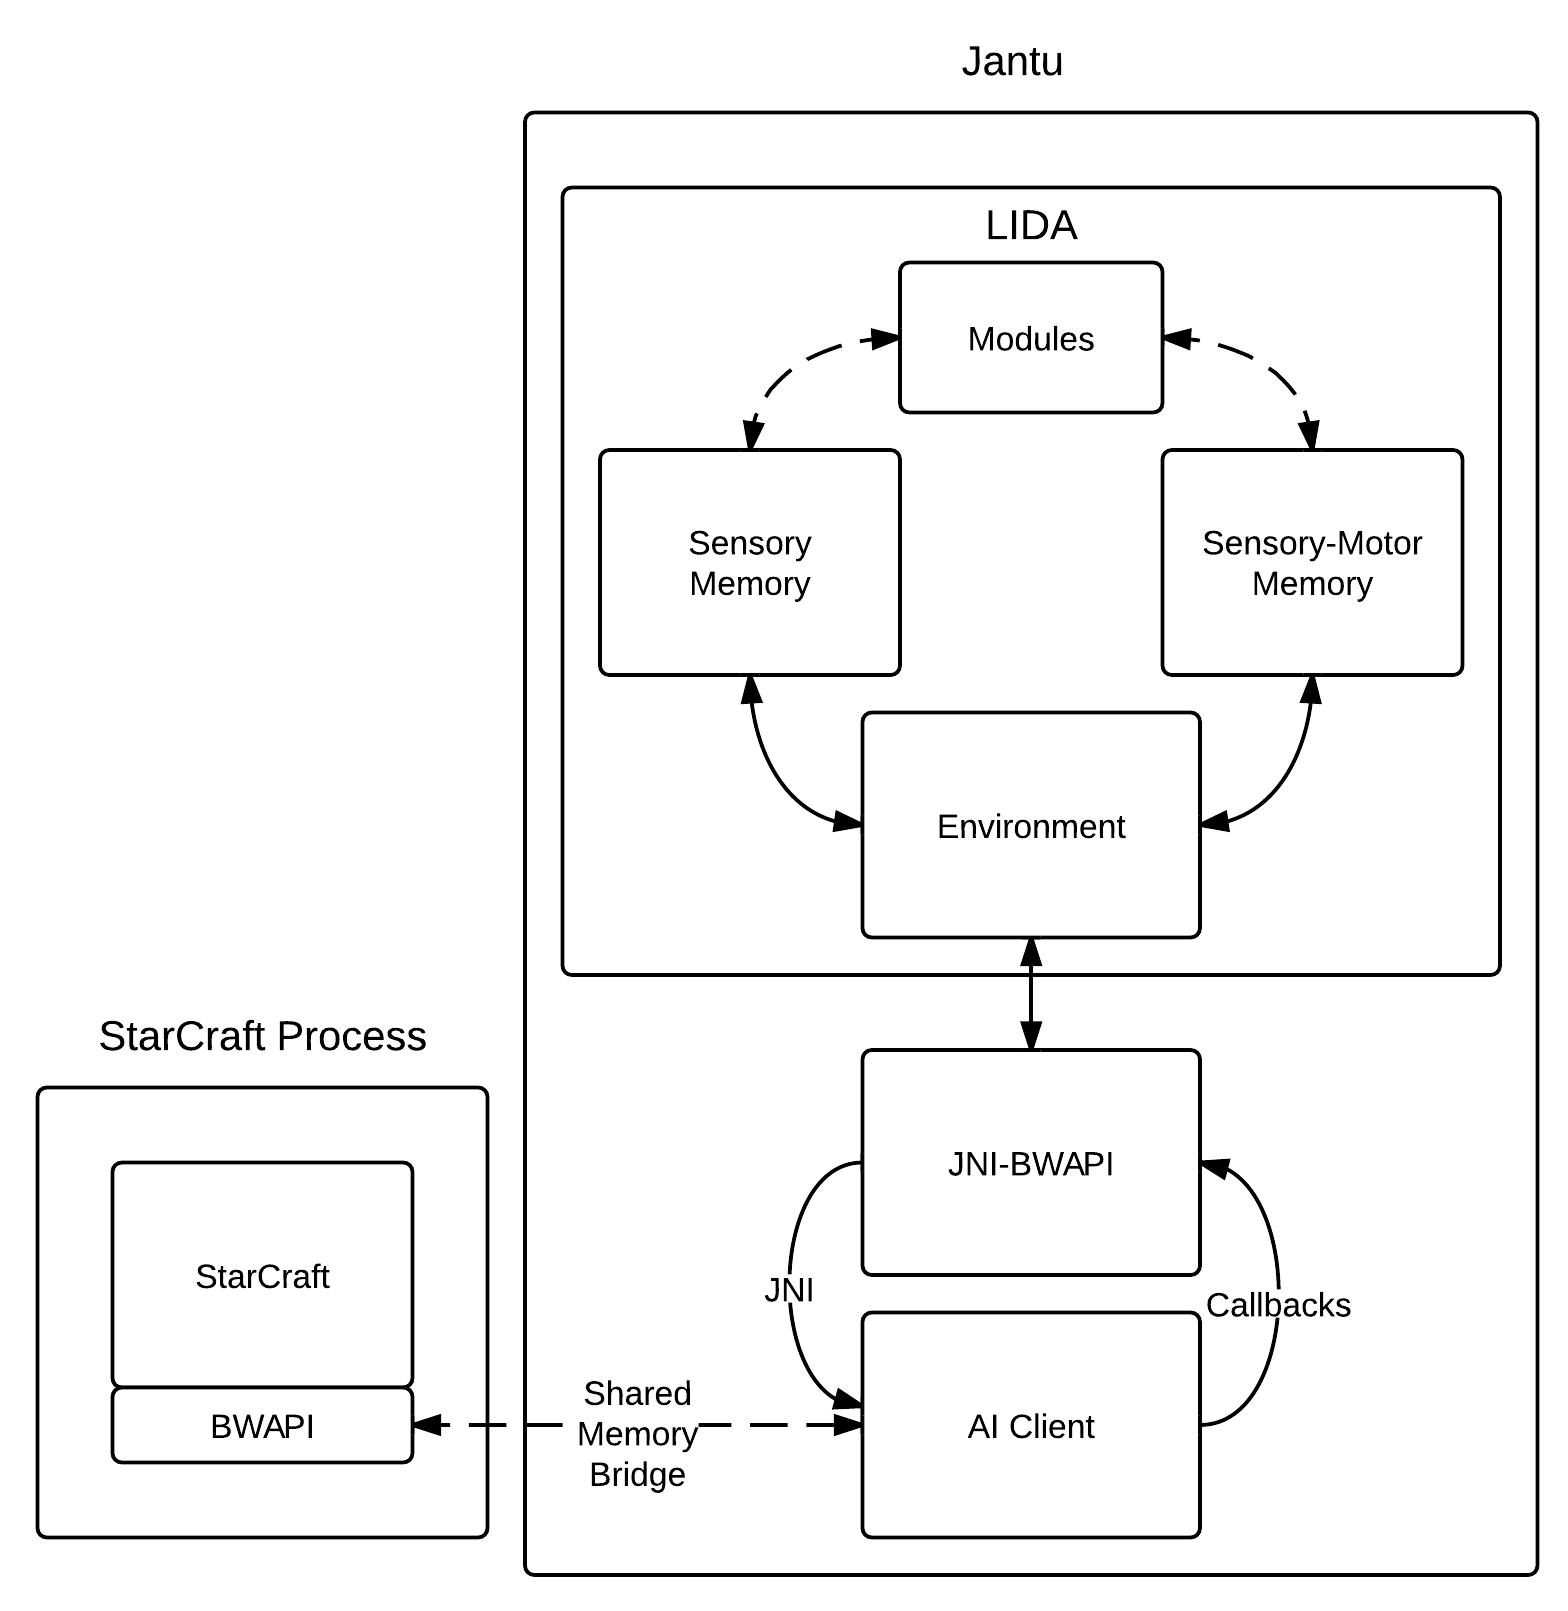
\includegraphics[scale=1.0]{graphics/jantu.png}
\caption{A general architecture overview of Jantu}
\label{fig:jantu}
\end{figure}

Figure \ref{fig:jantu} shows a general overview of the Jantu bots architecture, which consists of 3 main parts. In the Starcraft process the game it self runs together with BWAPI injected into the game client. Since this is all running in c++ and we are using the Java interface for BWAPI our code is run in a separate process that communicates with the Starcraft process using a shared memory bridge, this enables JNI-BWAPI to make calls to BWAPI and retrieve information back across the bridge. 

In the Jantu process JNI-BWAPI is running together with the LIDA framework. In order to integrate the LIDA framework with JNI-BWAPI we setup the framework first with the configurations we needed to get it up and running. This involves describing and structuring the modules you need in different XML configuration files. Also in these files we configure what kind of information that will be possible to use and transmit internally in the LIDA framework. 

JNI-BWAPI consists of different models and types that represent Starcraft information like units and buildings together with a lot of native functions that can be called to communicate with BWAPI. So we integraded this with LIDA by using a custom implementation of the Environment class in LIDA. This class becomes the interface between the domain specific modules of LIDA, the sensory memory and sensory-action memory, and JNI-BWAPI. 

\section{Detectors}
\label{sec:detectors}
Feature detectors is how LIDA perceives it's environment and identifies important aspects of the current game state. They are task that are run at specific intervals and parses the game state at that time in order to identify a given feature that can later be used in different modules in LIDA recognize thoughts and concepts. Each detector usually only identifies one specific feature, but it is possible for one detector to identify several features of they are of the same type. 

These are the detectors we implemented: 
\begin{itemize}
\item \textbf{IdleWorkerFeatureDetector} \\
This feature detector identifies worker units that doesn't have a job, a worker could be gathering resources, constructing buildings or scouting. But for efficiency it should be doing something at all times. 
\item \textbf{LarvaFeatureDetector} \\
This feature detector identifies larvae that are ready to be morphed into units. This is the only way Zerg can create units and when no larvae are available they can't create any more units until more larvae spawn. 
\item \textbf{ResourceFeatureDetector} \\
This feature detector identifies what type of units and buildings that we currently have enough resources available to create. This can be buildings we can construct, units we can morph or upgrades that we can research. 
\item \textbf{SupplyBlockFeatureDetector} \\
This feature detector identifies when we are getting close to being supply blocked, that means that we can't build any more units because another supply-granting building/unit is created.
\item \textbf{UnsaturatedResourcesFeatureDetector} \\
This feature detector identifies whether or not our available resource nodes have are saturated with enough workers that are gathering them. This can be used to decide if we need to build more workers or not.
\end{itemize}

Feature detectors can be created that detect almost every aspect of the game, and they can be everything from simply detecting the existence of specific units or game elements to more complex detectors that detect army compositions or enemy tactics and strategies. The more of them you implement the more advanced concepts you can identify and that opens up more advanced strategies you can perform yourself. 

\section{Action Execution}
\label{sec:actionexecution}
Action are executed with commands!

%!TEX root = main.tex

\chapter{Results}
This chapter presents results of how our implementation performed
\section{Architecture}
\label{sec:architecture}

\section{In-game performance}

\section{}
%!TEX root = main.tex

\chapter{Evaluation}
In this chapter we conclude our work by looking at the goals defined in the
introduction, and evaluate the results.
Section \ref{sec:evalres} evaluates the results of the project.
Section \ref{sec:conclusion} contains the final conclusion for the project and this report. 
Section \ref{sec:futurework} contains our thoughts on future implementation and improvements of our solution.


\section{Evaluation of Agent Performance}
While our agent makes poor decisions, this seems to stem mostly both from a lack of complex learning abilities, and from a lack of basic behaviours and feature detectors.

For instance, our agent does not detect the presence of enemy units at all, and we therefore rely on the built-in auto attack of enemy units for protection of our base. This often leads to ``base-trades'', where we are able to destroy the enemy base, but are unable to protect our own.

We also lack any kind of advanced microing behaviour, which means we utilize the units produced very badly. One observed behaviour was simply marching a long line of zealots into the line of fire of a canon, so they were cut down one by one. A more effective strategy here would be to group them up beforehand, so at least some of them would be able to reach the canon and possibly kill it.

Another issue is that our bot only builds one particular unit. This makes it very easy for a human to counter, for example with air units, which the zealots are unable to attack.

Another pretty grave flaw in our agents behaviour is that it never expands to several bases. While this made things easier to implement (positioning of units etc. became trivial), it means that if we don't win quickly, we will run out of minerals, and we will be at a severe economic disadvantage if/when the opponent expands to several bases.

But while the actual performance of the agent is not at a high-level, we can see that it is already working in a human-like fashion, switching conscious attention between the things that need to be done, and acting on it.

\section{Evaluation of Implementation}
\label{sec:evalres}
Our motivation for this project was to create an agent, using LIDA, that could play StarCraft: Brood War, which we did by implementing a simple proof of concept agent using the LIDA framework. We also discovered some of the problems inherent in the use of this cognitive architecture for this domain.

While the performance of the agent itself left a lot to be desired, the work we implemented for our agent we believe will massively simplify the work of anyone else intending to do something similar. Our domain-specific classes should provide everything needed for any kind of agent using the LIDA framework for StarCraft: Brood War, and our implemented feature detectors and behaviour should be a good starting point, as well as a good example for other feature detectors and behaviours one needs to implement.

\section{Conclusion}
\label{sec:conclusion}
We succeded in achieving what we set out to do, and while the in-game performance was not excellent, we think it is a very good starting point for any future work in this area.

\section{Future Work}
\label{sec:futurework}
We believe that there are several areas to be worked on. Implementing more feature detectors, and more behaviours, might be the easiest and obvious way to go forward. Obviously missing behaviour is for example grouping and managing the individual units better, expanding to extra bases for additional income, as well as more complex build orders, instead of the extremely simple timing attack implemented in our bot.

Replacing the rule-based action selection module with a more advanced approach is also something to look into. Version 1.2 of the LIDA framework replaces the default rule-based action selection with a behaviour network, based on Maes' behaviour network.\cite{maes1989right}

A more significant change would be to use the various memory modules available more actively.\cite{franklin2007lida}. This could help with for example letting the bot remember more about the state of the game, for example if it has already built the necessary building necessary for a certain unit, or remember build orders (learned from earlier games).

Learning could also be implemented at several other levels, not just as long-term memory.

\endrefsection

\cleardoublepage
\phantomsection
\addcontentsline{toc}{chapter}{Bibliography}
\printbibliography

\end{document}
